% Charlotte Geiger - Manuel Lippert - Leonard Schatt
% Physikalisches Praktikum

% Teilauswertung 2

\section{Mie-Streuung}

\subsection*{Relative Streuung}

In diesem Versuchsteil wir die Mie-Streuung an drei unterschielichen Proben durchgeführt. Durch diese versucht man Informationen über die 
Probe in Erfahrung zu bringen. Dies funktioniert, da beim Streuen ein Bild des reziproken Raumes abgebildet wird. Dieses enthält Informationen über 
typische Abstände in der Probe. \\
Brechnet wurden die relative Streuung der Proben $\Delta S$ bezüglich der Leerprobe. Dabei wurden die Fehler nach Fehlerfortpflanzungsgesetz berechnet.
\begin{gather}
    \Delta S = S_{Probe}- S_{Wasser}\\
    s_{\Delta} = \sqrt{(s_{S_{Probe}})^2+(s_{S_{Wasser}})^2}
\end{gather}

%begin{co
%begin{tabular}{lrrrrrrrr}
%   \toprule
%   {} &  Phi/Grad &  $\Delta S_{\parallel 1}$ &  $s_{\Delta S_{\parallel 1}}$ &  $\Delta S_{\parallel 2}$ &  $s_{\Delta S_{\parallel 1}}$ &  $\Delta S_{\perp  1}$ &  $s_{\Delta S_{\perp  1}}$ &  \$\textbackslash Delta S\$s2 \\
%   \midrule
%   1  &        30 &        170.96 &        2.828427 &         63.36 &        2.061553 &        268.96 &        5.024938 &        277.49 \\
%   2  &        35 &        150.67 &        2.828427 &         55.18 &        2.061553 &        260.70 &        5.024938 &        258.27 \\
%   3  &        40 &        129.64 &        2.061553 &         51.65 &        0.707107 &        254.36 &        5.024938 &        245.90 \\
%   4  &        45 &        106.25 &        2.061553 &         40.01 &        0.707107 &        248.18 &        5.024938 &        218.74 \\
%   5  &        50 &         88.81 &        2.061553 &         34.70 &        0.707107 &        242.77 &        5.024938 &        206.87 \\
%   6  &        55 &         73.15 &        2.061553 &         25.53 &        0.707107 &        242.72 &        5.024938 &        198.78 \\
%   7  &        60 &         53.94 &        2.061553 &         18.39 &        0.707107 &        238.81 &        5.024938 &        185.00 \\
%   8  &        65 &         38.70 &        2.061553 &         11.64 &        0.707107 &        232.88 &        5.024938 &        207.30 \\
%   9  &        70 &         27.94 &        0.707107 &          8.11 &        0.707107 &        207.53 &        5.024938 &        186.20 \\
%   10 &        75 &         18.69 &        0.707107 &          5.03 &        0.707107 &        200.37 &        5.024938 &        183.93 \\
%   11 &        80 &         11.68 &        0.707107 &          2.87 &        0.707107 &        192.56 &        5.024938 &        172.14 \\
%   12 &        85 &          7.00 &        0.707107 &          1.55 &        0.707107 &        184.73 &        5.024938 &        155.62 \\
%   13 &        90 &          4.75 &        0.707107 &          0.89 &        0.707107 &        181.55 &        5.024938 &        157.35 \\
%   14 &        95 &          4.80 &        0.707107 &          0.88 &        0.707107 &        179.78 &        5.024938 &        162.23 \\
%   15 &       100 &          6.33 &        0.707107 &          1.45 &        0.707107 &        177.28 &        5.024938 &        155.50 \\
%   16 &       105 &          9.40 &        0.707107 &          2.78 &        0.707107 &        173.91 &        5.024938 &        142.76 \\
%   17 &       110 &         15.74 &        0.707107 &          5.51 &        0.707107 &        171.66 &        5.024938 &        130.69 \\
%   18 &       115 &         23.26 &        0.707107 &          9.53 &        0.707107 &        175.19 &        5.024938 &        135.14 \\
%   19 &       120 &         28.67 &        0.707107 &          9.02 &        0.707107 &        170.18 &        5.024938 &        128.37 \\
%   20 &       125 &         36.98 &        0.707107 &         11.47 &        0.707107 &        161.47 &        5.024938 &        123.30 \\
%   21 &       130 &         47.32 &        2.061553 &         14.08 &        0.707107 &        160.60 &        5.024938 &        125.74 \\
%   22 &       135 &         51.43 &        2.061553 &         17.88 &        0.707107 &        139.31 &        5.385165 &        117.49 \\
%   23 &       140 &         63.91 &        2.061553 &         21.26 &        0.707107 &        139.15 &        5.385165 &        110.99 \\
%   24 &       145 &         68.89 &        2.828427 &         14.23 &        2.828427 &        136.08 &        5.385165 &        134.05 \\
%   25 &       150 &         80.43 &        2.828427 &         24.50 &        2.828427 &        121.50 &        5.385165 &        134.82 \\
%   \bottomrule
%   \end{tabular}
    
\textcolor{red}{Alle Werte in Tabelle \ref{Streuparameter} der relativen Streuung und ihrer  Fehler werden in mV angegeben.}   
    
\begin{table}[ht]
    \centering
    \captionsetup{justification=centering,margin=2cm}
    \begin{tabular}{lrrrrrrrrr}
        \toprule
        {} &  $\phi$ in $^{\circ}$   &  $\Delta S_{\parallel 1}$ &  $s_{\Delta S_{\parallel 1}}$ &  $\Delta S_{\parallel 2}$ &  $s_{\Delta S_{\parallel 1}}$ &  $\Delta S_{\perp  1}$ &  $s_{\Delta S_{\perp  1}}$ & $\Delta S_{\perp  2}$ &   $s_{\Delta S_{\perp 2}}$ \\
        \midrule
        1  &        30 &        170.96 &            2.83 &         63.36 &            2.06 &        268.96 &            5.02 &        277.49 &            5.02 \\
    2  &        35 &        150.67 &            2.83 &         55.18 &            2.06 &        260.70 &            5.02 &        258.27 &            5.02 \\
    3  &        40 &        129.64 &            2.06 &         51.65 &            0.71 &        254.36 &            5.02 &        245.90 &            5.02 \\
    4  &        45 &        106.25 &            2.06 &         40.01 &            0.71 &        248.18 &            5.02 &        218.74 &            5.02 \\
    5  &        50 &         88.81 &            2.06 &         34.70 &            0.71 &        242.77 &            5.02 &        206.87 &            5.02 \\
    6  &        55 &         73.15 &            2.06 &         25.53 &            0.71 &        242.72 &            5.02 &        198.78 &            5.02 \\
    7  &        60 &         53.94 &            2.06 &         18.39 &            0.71 &        238.81 &            5.02 &        185.00 &            5.02 \\
    8  &        65 &         38.70 &            2.06 &         11.64 &            0.71 &        232.88 &            5.02 &        207.30 &            5.02 \\
    9  &        70 &         27.94 &            0.71 &          8.11 &            0.71 &        207.53 &            5.02 &        186.20 &            5.02 \\
    10 &        75 &         18.69 &            0.71 &          5.03 &            0.71 &        200.37 &            5.02 &        183.93 &            5.02 \\
    11 &        80 &         11.68 &            0.71 &          2.87 &            0.71 &        192.56 &            5.02 &        172.14 &            5.02 \\
    12 &        85 &          7.00 &            0.71 &          1.55 &            0.71 &        184.73 &            5.02 &        155.62 &            5.02 \\
    13 &        90 &          4.75 &            0.71 &          0.89 &            0.71 &        181.55 &            5.02 &        157.35 &            5.02 \\
    14 &        95 &          4.80 &            0.71 &          0.88 &            0.71 &        179.78 &            5.02 &        162.23 &            5.02 \\
    15 &       100 &          6.33 &            0.71 &          1.45 &            0.71 &        177.28 &            5.02 &        155.50 &            5.02 \\
    16 &       105 &          9.40 &            0.71 &          2.78 &            0.71 &        173.91 &            5.02 &        142.76 &            5.02 \\
    17 &       110 &         15.74 &            0.71 &          5.51 &            0.71 &        171.66 &            5.02 &        130.69 &            5.02 \\
    18 &       115 &         23.26 &            0.71 &          9.53 &            0.71 &        175.19 &            5.02 &        135.14 &            5.02 \\
    19 &       120 &         28.67 &            0.71 &          9.02 &            0.71 &        170.18 &            5.02 &        128.37 &            5.02 \\
    20 &       125 &         36.98 &            0.71 &         11.47 &            0.71 &        161.47 &            5.02 &        123.30 &            5.02 \\
    21 &       130 &         47.32 &            2.06 &         14.08 &            0.71 &        160.60 &            5.02 &        125.74 &            5.02 \\
    22 &       135 &         51.43 &            2.06 &         17.88 &            0.71 &        139.31 &            5.39 &        117.49 &            5.39 \\
    23 &       140 &         63.91 &            2.06 &         21.26 &            0.71 &        139.15 &            5.39 &        110.99 &            5.39 \\
    24 &       145 &         68.89 &            2.83 &         14.23 &            2.83 &        136.08 &            5.39 &        134.05 &            5.39 \\
    25 &       150 &         80.43 &            2.83 &         24.50 &            2.83 &        121.50 &            5.39 &        134.82 &            5.39 \\
        \bottomrule
    \end{tabular}

    \caption{Intensität der relativen Streuung von Probe 1 und 2 bei Einstrahlung von parallel bzw. senkrecht polarisiertem Licht}
    \label{Streuparameter}
\end{table}

\begin{figure}[ht]
    \captionsetup{justification=centering,margin=2cm}
    \centering
    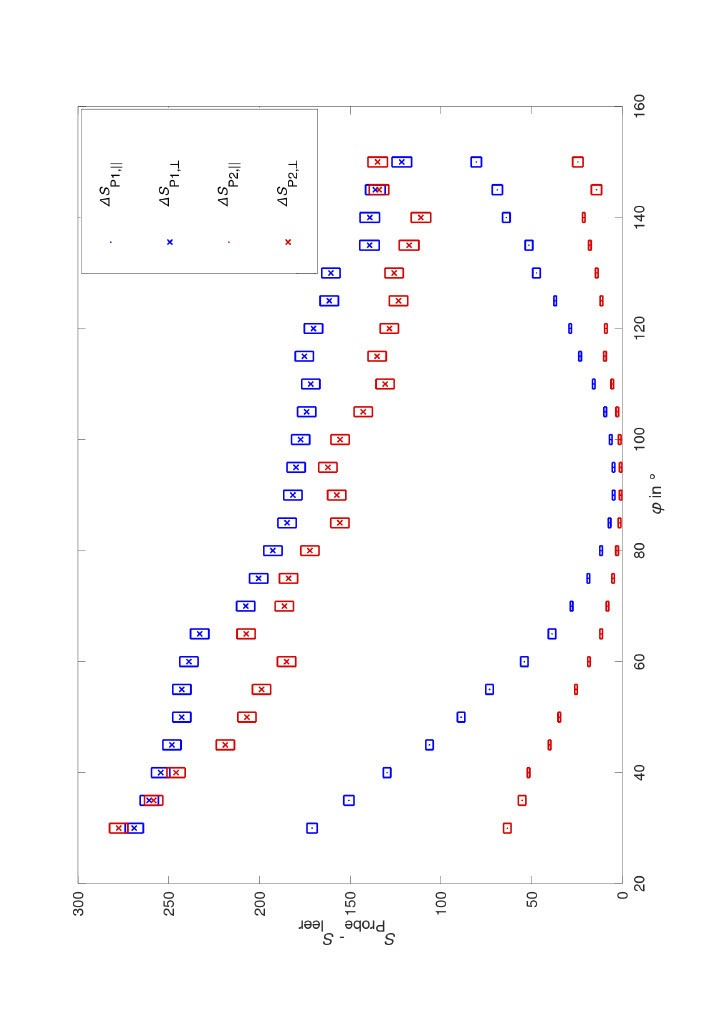
\includegraphics[width = \linewidth]{Bilder/RelativeStreuung.jpg}
    \caption{Relative Streuung von Probe 1 und Probe 2 bei sekrechter und paralleler Polarisation}
\end{figure}


\subsection*{Polarisationsgrad}

Als Nächstes wird der Polarisationsgrad betrachtet. Dabei wird der Fehler mit Fehlerfortpflanzung berechnet anhand der folgenden Formeln:
\begin{gather}
    P = \frac{\Delta S_{\perp}-\Delta S_{\parallel}}{\Delta S_{\perp} + \Delta S_{\parallel}}\\
    s_P = \frac{2}{(\Delta S_{\perp} + \Delta S_{\parallel})^2}\sqrt{(\Delta S_{\parallel} s_{\Delta S_{\perp}})^2+ (\Delta S_{\perp} s_{\Delta S_{\parallel}})^2}
\end{gather}
Im Gegensatz dazu verhält sich Rayleighstreuung folgendermaßen:
\begin{equation*}
    P_{Rayleigh} = \frac{\sin[2](\phi)}{1+ \cos[2](\phi)}.
\end{equation*}

\begin{center}
    \begin{table}
    \captionsetup{justification=centering,margin=2cm}
    \centering
    \begin{tabular}{lrrrrr}
        \toprule
        {} &  $P_1$ &   $s_{P_1}$ & $P_2$& $s_{P_2}$ \\
        \midrule
         1 &  0.22 &  0.01 &  0.63 &  0.01 \\
         2 &  0.27 &  0.01 &  0.65 &  0.01 \\
         3 &  0.32 &  0.01 &  0.65 &  0.01 \\
         4 &  0.40 &  0.01 &  0.69 &  0.01 \\
         5 &  0.46 &  0.01 &  0.71 &  0.01 \\
         6 &  0.54 &  0.01 &  0.77 &  0.01 \\
         7 &  0.63 &  0.01 &  0.82 &  0.01 \\
         8 &  0.72 &  0.01 &  0.89 &  0.01 \\
         9 &  0.76 &  0.01 &  0.92 &  0.01 \\
        10 &  0.83 &  0.01 &  0.95 &  0.01 \\
        11 &  0.89 &  0.01 &  0.97 &  0.01 \\
        12 &  0.93 &  0.01 &  0.98 &  0.01 \\
        13 &  0.95 &  0.01 &  0.99 &  0.01 \\
        14 &  0.95 &  0.01 &  0.99 &  0.01 \\
        15 &  0.93 &  0.01 &  0.98 &  0.01 \\
        16 &  0.90 &  0.01 &  0.96 &  0.01 \\
        17 &  0.83 &  0.01 &  0.92 &  0.01 \\
        18 &  0.77 &  0.01 &  0.87 &  0.01 \\
        19 &  0.71 &  0.01 &  0.87 &  0.01 \\
        20 &  0.63 &  0.01 &  0.83 &  0.01 \\
        21 &  0.54 &  0.02 &  0.80 &  0.01 \\
        22 &  0.46 &  0.02 &  0.74 &  0.01 \\
        23 &  0.37 &  0.02 &  0.68 &  0.02 \\
        24 &  0.33 &  0.03 &  0.81 &  0.04 \\
        25 &  0.20 &  0.03 &  0.69 &  0.03 \\
        \bottomrule
    \end{tabular}
    \caption{Polarisationsgrad von Probe 1 und Probe 2 mit Fehler} 
    \label{PolarisationsgradTabelle}  
    \end{table}     
\end{center}

\begin{figure}[h]
    \captionsetup{justification=centering,margin=2cm}
    \centering
    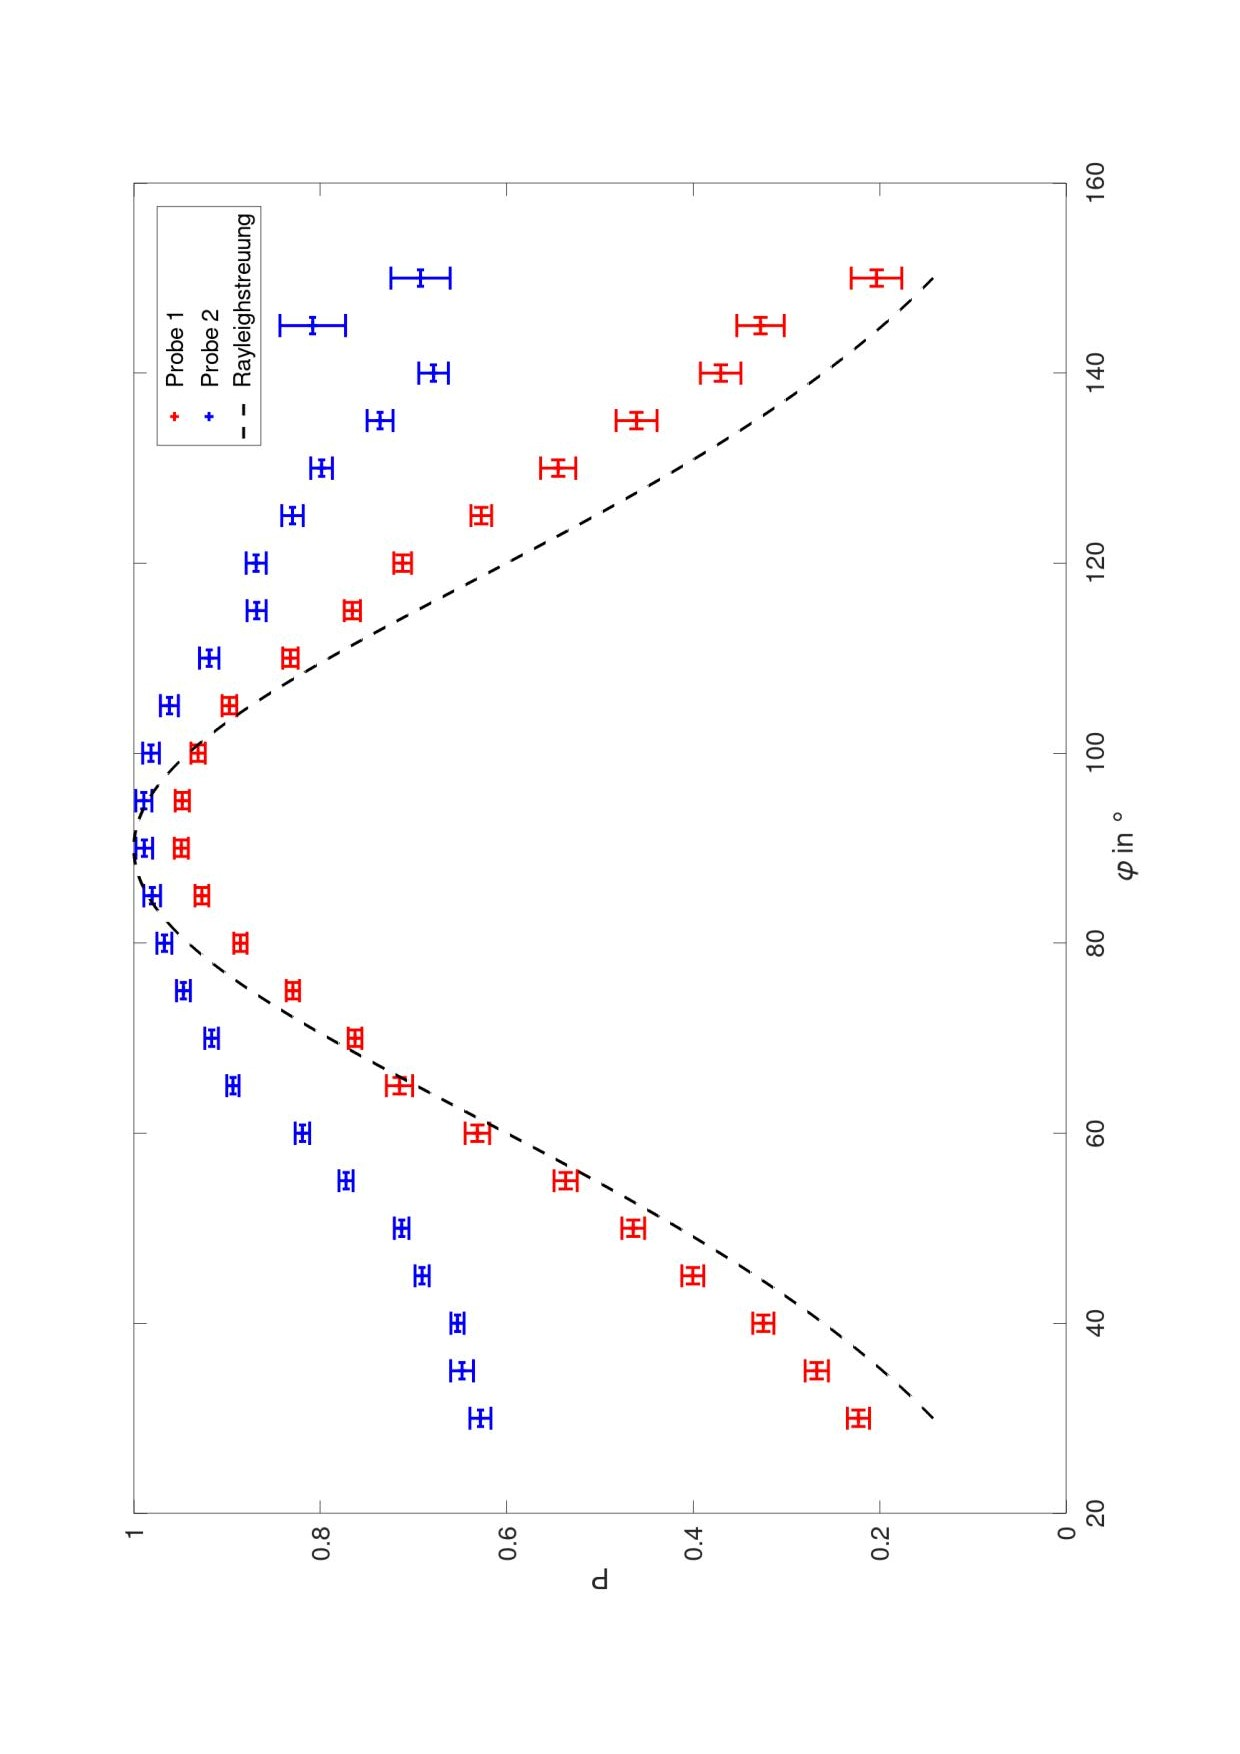
\includegraphics[width = \linewidth]{Bilder/Polarisattionsgrad.jpg}
    \caption{Polarisationsgrad der Probe 1 und Probe 2 aufgetragen mit der theoretischen Rayleighstreuung}
    \label{PolarisationsgradBild}
\end{figure}




Erstmal fällt in Grafik \ref{PolarisationsgradBild} auf, dass bei Probe 2 die Messung sehr dubios scheint. Die ungefähre Form der Kurve 
stimmt zwar, jedoch beginnen die Werte erst bei circa 0,6. Das bei der Messung irgend ein Fehler vorliegt, ist uns auch wärend das Versuches schon aufgefallen. Das 
riesige "schwanken" in der Messung, was alles überlagerte, hat leider ein korrekte Messen erschwert.\\
In der Grafik sieht man sehr schön, dass das Maximum bei beiden Kurven relativ genau bei 90$^{\circ}$ liegt. Die Kurven für beide Proben, vorallem vom Probe 1 
weisen eine beeindruckende Symmetrie auf bezüglich einer Achse durch 90$^{\circ}$.

\subsection*{Asymmetriefaktor}

Da in der Versuchsbeschreibung der Asymmetriefaktor $X$ in einer Tabelle für $\phi = 45^{\circ}$ gegeben ist. Wir verwenden dafür jeweils $S_{\perp}$, was jedoch an sich irrelevant sein sollte, 
da $X$ eine von der Polarisation unabhängige Größe ist.
\begin{gather*}
    \phi = 45^{\circ}\\
    X = \frac{S(\phi)}{S(\pi - \phi)}\\
    s_X = \sqrt{(\frac{s_S (\phi)}{S(\pi-\phi)})^2+(\frac{S(\phi) \cdot s_S (\pi-\phi)}{(S(\pi-\phi))^2})^2}
\end{gather*}
Berechnet man diese erhält man:\\
\begin{center}
    \begin{tabular}{cc}
        $X_1$ = 1,7814945 & $s_{X_{1}}$ = 0,07777833\\
        $X_2$ = 1,8617754 & $s_{X_{2}}$ = 0,09550227\\
    \end{tabular}
\end{center}
\begin{center}
    \minibox[frame]{$X_1$ = 1,78$\pm$0,08 \\
     $X_2$ = 1,86$\pm$ 0,09}
\end{center}
In der Tabelle im Skript sind als Referenzwerte die Werte für $\frac{D}{\lambda_M}$ gegeben, wobei 
$D$ die Teilchengröße und $\lambda_M$ die Wellenlänge im Medium. Das Medium, hier Wasser, hat einen Brechungsindex 
$n_{Wasser}$ = 1,33. 
Die Wellenlänge im Medium ergibt sich wiefolgt:
\begin{gather*}
    \lambda_{Vakuum} = 632,8 \mathrm{nm} \\
    \lambda_M = \lambda_{Wasser} = \frac{\lambda_{Vakuum}}{n_{Wasser}}\\
    \rightarrow \lambda_{Wasser} = 475,79\mathrm{nm}
\end{gather*}
Da in der Tabelle die von uns errechneten Werte nicht exakt tabuliiert sind, können wir nur Zwischenwerte abschätzen. Für diese nehmen wir einen Fehler von 0,005 als Ablesefehler an. 
\begin{center}
    \begin{tabular}{cc}
        Probe 1: & $\frac{D}{\lambda_M}$ = 0,31\\
        Probe 2: & $\frac{D}{\lambda_M}$ = 0,33\\
    \end{tabular}
\end{center}
Die Teilengröße ergibt sich trivialer Weise mit 
\begin{gather*}
    D = \frac{D}{\lambda_m}\lambda_M\\
    s_D \approx 0,005*\lambda_M = 3,164\mathrm{nm}
\end{gather*}
\begin{center}
    \centering
    $\Rightarrow$ \minibox[frame]{$D_1$ = (147$\pm$3)nm\\$D_2$ = (157$\pm$3)nm}
\end{center}
Die mit dem bloßen Auge nicht sichtbaren Schwebstoffe in dem Wasser sind erstaunlich klein. Die Teilchen haben eine Größe vom mur wenigen Nanometern. 
Dies ist in der Tat erstaunlich, da wir damit in der Größenordnung einzelner langkettiger Polymermolekülen sind. Dieser Versuch scheint also ein sehr gute Methode zu sein um 
Strukturen auf kleinen Skalen aufzulösen. Verbessern könnte man die Methodik noch, indem man höherenergetische Strahlung nimmt. Dann würde man es GISAX, SAX, GIWAX oder Wax nennen. Diese Methoden 
sind vorallem bei Strukturanalysen, beispielsweise im Bereich der Halbleiterphysik sehr verbreitet.